\documentclass{jsreport}
\input preamble.tex
\begin{document}
\chapter{非協力ゲーム理論の基礎}
\section{ゲーム理論とは}
ゲームは次の3つの要素を持つ.
\begin{itemize}
  \item 複数の行動主体(プレイヤー,エージェント).
  \item 各主体のとりうる行動(戦略)\footnote{行動はある1つの行動を表し,戦略は,どのようなルールで行動をするかを表す.ゲームにおいては同じ意味で用いられることもある.}の集合.
  \item 各主体の結果に対する評価(利得,効用)\footnote{利得は純粋なスコア,効用な具体的な対象が見えるもののイメージ.}.
\end{itemize}

これらを用いて社会や経済の持つ基本的な特性を表すことができる.複数の主体がどのような行動をとるかによって,全体が決まる.ゲーム理論では,複数の意思決定主体からなる社会の有り様や,主体の行動を研究する\footnote{状況(given)をゲームとして記述することで分析を行う.これを逆に用いると制御系設計ができる.}.

ゲーム理論の中に非協力ゲーム理論がある.これは,各主体の利益が必ずしも一致せず,競合状態にあるものを考えている.つまり,各主体は自分の利益のみを考え,利己的に行動する.ただし,他の主体と完全に対立するときもあれば,他の主体の利益と自分の利益が一致するときもある\footnote{このことから,協力ゲームは非協力ゲームで記述できるとされている.}.

非協力ゲームにおける古典的な仮定として,「完全情報」と「完全合理性」がある.完全情報とは,エージェントがゲームの情報(3要素)を完全に分かっているというものである.完全合理性とは,自身の保有する情報全てを用いて,自身の利益の最大化を実現することである.分散制御では,情報が完全に得られないこともある.近年では,この仮定を緩めることも多い.

\section{純粋戦略}
\subsection{戦略型ゲーム}
戦略型ゲームは次のように定義される.
\begin{screen}
  \begin{defi}[戦略型ゲーム]
  戦略型ゲーム$G = (\mathcal{N}, \mathcal{A}, U)$は次の3要素で定義される.
  \begin{itemize}
    \item $\mathcal{N} = \{1, 2, \ldots, n\}$
    \begin{itemize}
      \item エージェントの集合.
    \end{itemize}
    \item ${\cal A} = \times_{i \in N} {\cal A}_i$
    \begin{itemize}
      \item エージェントの行動プロファイルの集合.
    \end{itemize}
    \item $U \, : \, {\cal A} \rightarrow \mathbb{R}^n$
    \begin{itemize}
      \item 全エージェントの利得関数.
      \item 行動プロファイル$a \in {\cal A}$に対して,利得ベクトル
      $U(a) = (U_1(a), U_2(a), \ldots, U_n(a))$
      を割り当てる.
    \end{itemize}
  \end{itemize}
  \end{defi}
\end{screen}

ただし,
\begin{itemize}
  \item ${\cal A}_i = \{1, 2, \ldots, m_i\}$
  \begin{itemize}
    \item エージェント$i \in N$の選択可能な行動(純粋戦略)の集合(行動インデックス集合).
  \end{itemize}
  \item $U_i \, : \, {\cal A} \rightarrow \mathbb{R}$
  \begin{itemize}
    \item エージェント$i \in N$の(純粋戦略)利得関数\footnote{定義域が${\cal A}$ (エージェントのの行動プロファイル集合)であることからも,エージェント$i \in N$が得る利得は他のエージェントの行動にも依存することがわかる.}.
    \item 各エージェントは利得を最大化するように戦略を選択する.
  \end{itemize}
\end{itemize}
である.

特に,2人ゲームのときは利得行列$A, B$によってゲームを表現することができる.$e_{m_i}^k \in \mathbb{R}^{m_i}$を第$k$要素が$1$の$m_i$次元単位ベクトルとすると,$k \in {\cal A}_1, h \in {\cal A}_2$に対して,
\begin{equation}
  U_1(k, h) = (e_{m_1}^k)^{\mathrm{T}} A e_{m_2}^{h}, \; \; U_2(k, h) = (e_{m_1}^k)^{\mathrm{T}} B e_{m_2}^{h} \nonumber
\end{equation}
である.$U_1(k, h)$は,1人目が$k$,2人目が$h$を取ったときの1人目の利得であり,$U_2(k, h)$は1人目が$k$,2人目が$h$を取ったときの2人目の利得である.

ここで,「囚人のジレンマ」を例に2人ゲームの利得行列について説明する.
\begin{itemize}
  \item エージェント
  \begin{itemize}
    \item $N = \{1, 2\}$ (2人の囚人)
  \end{itemize}
  \item 行動集合
  \begin{itemize}
    \item ${\cal A}_1 = {\cal A}_2 = \{協力, 裏切り\}$
  \end{itemize}
  \item 利得\footnote{一般に2人ゲームの利得を表す表においては,行が1人目のエージェント,列が2人目のエージェントを表す.1人目のエージェントを行プレイヤー,列が2人目のエージェントを列プレイヤーともいう.表において,$\cdot,\cdot$は,左側が1人目のエージェントの得る利得,右側が2人目のエージェントの得る利得を表す.}
  \begin{table}[H]
  \centering
    \begin{tabular}{c|c|c}
          & 協力 & 裏切り  \\ \hline
      協力 & $-1, -1$ & $-5, 0$ \\ \hline
      裏切り & $0, -5$ & $-2, -2$ \\
    \end{tabular}
  \end{table}
  \item 利得行列
  \begin{equation}
    A = \left(
    \begin{array}{cc}
      -1 & -5 \\
      0 & -2
    \end{array}
    \right), \; \; B = \left(
    \begin{array}{cc}
      -1 & 0 \\
      -5 & -2
    \end{array}
    \right) \nonumber
  \end{equation}
\end{itemize}

\subsection{最適反応とナッシュ均衡}
次に,最適反応について定義する.最適反応とは,他のエージェントの行動を固定したとき,エージェント$i$が取りうる全ての行動の中で最も利得が高くなる(つまり,最適な)行動である.最適反応は次のように定義される.
\begin{screen}
  \begin{defi}[最適反応]
    $a_i^{*} \in {\cal A}_i$が$a_{-i} = (a_1, \ldots, a_{i - 1}, a_{i + 1}, \ldots, a_n)$に対する(純粋)最適反応である:
    \begin{equation}
      \forall a_i \in {\cal A}_i, \; U_i(a_i^{*}, a_{-i}) \geq U_i(a_i, a_{-i}) \nonumber
    \end{equation}
  \end{defi}
\end{screen}
この定義は,
\begin{equation}
  U_i(a_i^{*}, a_{-i}) = \max_{a_i \in {\cal A}_i} U_i(a_i, a_{-i}) \nonumber
\end{equation}
と等価である.最適反応は1つとは限らないが,必ず存在する.

ゲーム理論における重要な概念にナッシュ均衡がある.これは,1人だけが行動を変更しても得することがない状況を表す\footnote{ある意味最適解であると考えることもできる.}.ナッシュ均衡は次のように定義される.
\begin{screen}
  \begin{defi}[(純粋戦略)ナッシュ均衡]
    $a^{*} \in {\cal A}$が(純粋戦略)ナッシュ均衡である:
    \begin{equation}
      \forall i \in \mathcal{N}, \forall a_i \in {\cal A}_i, \; \; U_i(a_i^{*}, a_{-i}^{*}) \geq U_i(a_i, a_{-i}^{*}) \nonumber
    \end{equation}
  \end{defi}
\end{screen}
この定義は,
\begin{equation}
  \forall i \in \mathcal{N}, \; \; U_i(a_i^{*}, a_{-i}^{*}) = \max_{a_i \in {\cal A}_i} U_i(a_i, a_{-i}^{*}) \nonumber
\end{equation}
と等価である.ナッシュ均衡は全てのエージェントが純粋戦略最適反応をとることを表す.つまり,全てのエージェントにとって「合理的」な解であり,ナッシュ均衡が実現されれば,全てのエージェントはそこから動かない.
ナッシュ均衡は1つとは限らず,存在しない場合もある.

ナッシュ均衡について,次の3つの2人ゲームの例で説明する.
\paragraph{囚人のジレンマ}
エージェントの集合を$\mathcal{N} = \{1, 2\}$,行動集合を${\cal A}_1 = {\cal A}_2 = \{協力, 裏切り\}$,利得を
\begin{table}[H]
\centering
  \begin{tabular}{c|c|c}
        & 協力 & 裏切り  \\ \hline
    協力 & $-1, -1$ & $-5, 0$ \\ \hline
    裏切り & $0, -5$ & $-2, -2$ \\
  \end{tabular}
\end{table}
とする.

エージェント1(行プレイヤー)について,エージェント2(列プレイヤー)の行動を「協力」に固定したときの最適反応\footnote{表の1列目に注目し,1行目と2行目のエージェント1の利得でより高い値のもの.}は「裏切り」,「裏切り」に固定したときの最適反応\footnote{表の2列目に注目し,1行目と2行目のエージェント1の利得でより高い値のもの.}は「裏切り」である.
エージェント2についても同様に考えると,エージェント1の行動を「協力」に固定したときの最適反応は「裏切り」,「裏切り」に固定したときの最適反応は「裏切り」である.よって,ナッシュ均衡は(裏切り,裏切り)である.

\paragraph{男女の争い}
エージェントの集合を$\mathcal{N} = \{1, 2\}$,行動集合を${\cal A}_1 = {\cal A}_2 = \{ボクシング, バレエ\}$,利得を
\begin{table}[H]
\centering
  \begin{tabular}{c|c|c}
        & ボクシング & バレエ  \\ \hline
    ボクシング & $2, 1$ & $-1, -1$ \\ \hline
    バレエ & $-1, -1$ & $1, 2$ \\
  \end{tabular}
\end{table}
とする.

最適反応は,「ボクシング」に対して「ボクシング」,「バレエ」に対して「バレエ」である.よって,ナッシュ均衡は(ボクシング,ボクシング),(バレエ,バレエ)である.

\paragraph{じゃんけん}
エージェントの集合を$\mathcal{N} = \{1, 2\}$,行動集合を${\cal A}_1 = {\cal A}_2 = \{グー, チョキ, パー\}$,利得を
\begin{table}[H]
\centering
  \begin{tabular}{c|c|c|c}
        & グー & チョキ & パー  \\ \hline
    グー & $0, 0$ & $1, -1$ & $-1, 1$  \\ \hline
    チョキ & $-1, 1$ & $0, 0$ & $1, -1$ \\ \hline
    パー & $1, -1$ & $-1, 1$ & $0, 0$ \\
  \end{tabular}
\end{table}
とする.

最適反応は,「グー」に対して「パー」,「チョキ」に対して「グー」,「パー」に対して「チョキ」である.よって,ナッシュ均衡は存在しない.

\section{混合戦略}
ここまでのゲームの定義は,エージェントがある行動を確率1で取る(純粋戦略)というものだった.ここでは,エージェントが行動集合からある確率で行動を選択するもの(混合戦略)における最適反応およびナッシュ均衡を定義する.

\subsection{混合戦略}
エージェント$i$の行動集合を${\cal A}_i = \{1, \ldots, m_i\}$とし,エージェント$i$が行動$j \in {\cal A}_i$をとる確率を並べたベクトルを$x_i = (x_i^1, \ldots, x_i^{m_i})^{\mathrm{T}}$とする.この$x_i$を混合戦略という.混合戦略$x_i$の集合
\begin{equation}
  X_i = \left\{x_i \, \left| \, \forall j \in {\cal A}_i \, x_i^{j} \geq 0, \, \sum_{k \in {\cal A}_i} x_i^{k} = 1\right.\right\} \nonumber
\end{equation}
は行動集合${\cal A}_i$上の確率分布である.この$X_i$は単位ベクトル$e_{m_i}^j$を頂点とする$m_i - 1$次元単位単体となる.

エージェント$i$の行動集合${\cal A}_i$が${\cal A}_i = \{1, 2\}$の例を考える($m_i = 2$).混合戦略を$x_i = (x_i^1, x_i^2)^{\mathrm{T}}$とすると,混合戦略$x_i$は,
線分$x_i^1 + x_i^2 = 1, \; 0 \leq x_i^1, x_i^2 \leq 1$上の点である(図\ref{fig:mixed}).
つまり,エージェント$i$の混合戦略の集合は,
\begin{equation}
  X_i = \{(x_i^1, 1 - x_i^1)^{\mathrm{T}} \, | \, 0 \leq x_i^1 \leq 1\} \nonumber
\end{equation}
と表される.
\begin{figure}[htb]
  \centering
  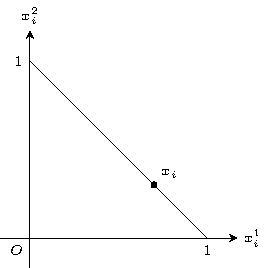
\includegraphics[clip, width=5cm]{./fig/graph_1.pdf}
  \caption{$1$次元単位単体(線分)}
  \label{fig:mixed}
\end{figure}


各エージェント$i$の混合戦略の集合$X_i$の直和
\begin{equation}
  X = \times_{i \in N} X_i \nonumber
\end{equation}
を混合戦略空間という.また,
\begin{itemize}
  \item $x \in X$
  \begin{itemize}
    \item 混合戦略プロファイル.
  \end{itemize}
  \item $C(x_i) = \{j \in {\cal A}_i \, | \, x_i^j > 0\}$
  \begin{itemize}
    \item $x_i \in X_i$のキャリア.
    \item 実際に使われる可能性のある行動の集合.
  \end{itemize}
\end{itemize}
である.

混合戦略の集合$X_i$について,
\begin{equation}
  \mathrm{int}(X_i) = \{x_i \in X_i, \, | \, \forall j \in {\cal A}_i \; x_i^j > 0\} \nonumber
\end{equation}
を$X_i$の内部といい\footnote{つまり,内部はキャリアと行動集合が一致するような混合戦略の集合である.},
\begin{equation}
  \mathrm{bd}(X_i) = \{x_i \in X_i \, | \, x_i \notin \mathrm{int}(X_i)\} \nonumber
\end{equation}
を$X_i$の境界という.$x_i \in \mathrm{int}(X_i)$を完全混合戦略(内部戦略)といい,$x \in \mathrm{int}(X) = \times_{i \in N} \mathrm{int}(X_i)$を完全混合プロファイル(内部プロファイル)という.

図\ref{fig:mixed}において,点$(x_i^1, x_i^2)^{\mathrm{T}} = (1, 0)^{\mathrm{T}}, \, (0, 1)^{\mathrm{T}}$は境界であり,それ以外の点は内部である.

\subsection{期待効用理論}
非協力ゲームにおいて,エージェントは期待利得を最大化しょうとする.戦略プロファイル$x \in X$で,行動プロファイル$a \in {\cal A}$が実際に起こる確率$x(a)$は,
\begin{equation}
  x(a) = \prod_{i \in \mathcal{N}} x_i^{a_i} \label{eq:xa}
\end{equation}
である.\eqref{eq:xa}は,エージェント$i \in \mathcal{N}$が行動$a_i \in A_i$を取る確率が$x_i^{a_i}$であり,行動プロファイル$a = (a_1, \ldots, a_n)$が起こる確率はこの積で表されることを示している.

エージェント$i$の利得の期待値を期待利得という.エージェント$i$の期待利得関数$u_i: X \to \mathbb{R}$は以下で定義される.
\begin{align}
  u_i(x) &\coloneqq x(a)U_i(a) \label{eq:def_exputil} \\
  &= \sum_{j \in A_i} x_i^j u_i(e_{m_i}^j, x_{-i}) \label{eq:exputil_sum}
\end{align}
\eqref{eq:def_exputil}は,エージェント$i$の期待利得が,エージェント$i$の利得の期待値であるという期待利得の定義である.\eqref{eq:exputil_sum}は,各エージェントの混合戦略に関して,各エージェントの期待利得は線形性を持つことを示している.
\subsection{戦略型ゲームの混合拡大}
混合拡大した戦略型ゲームは,以下のように定義される.
\begin{screen}
  \begin{defi}[戦略型ゲーム]
  戦略型ゲーム$G = (\mathcal{N}, X, u)$は次の3要素で定義される.
  \begin{itemize}
    \item $\mathcal{N} = \{1, 2, \ldots, n\}$
    \begin{itemize}
      \item エージェントの集合.
    \end{itemize}
    \item $X = \times_{i \in N} X_i$
    \begin{itemize}
      \item 混合戦略空間
      \begin{equation}
        X_i = \left\{x_i \, \left| \, \forall j \in \mathcal{A}_i \, x_i^j \geq 0, \sum_{k \in \mathcal{A}_i} x_i^k = 1\right.\right\} \nonumber
      \end{equation}
    \end{itemize}
    \item $u \, : \, X \rightarrow \mathbb{R}^n$
    \begin{itemize}
      \item 混合戦略プロファイル$x \in S$に対して,利得ベクトル
      $u(x) = (u_1(x), u_2(x), \ldots, u_n(x))$
      を割り当てる.
    \end{itemize}
  \end{itemize}
  \end{defi}
\end{screen}

特に,2人ゲームのときは利得行列$(A, B)$によってゲームが表現される.
\begin{align}
  u_1(x) &= \sum_{j \in \mathcal{A}_1} x_1^j u_1(e_{m_1}^j, x_2) = \sum_{j \in \mathcal{A}_1} \sum_{k \in \mathcal{A}_2} x_1^j x_2^k a_{jk} = x_1^{\mathrm{T}}Ax_2 \nonumber \\
  u_2(x) &= \sum_{j \in \mathcal{A}_1} \sum_{k \in \mathcal{A}_2} x_1^j x_2^k b_{jk} = x_1^{\mathrm{T}} B x_2 \nonumber
\end{align}
ここからも分かるように,純粋戦略は,ある戦略を確率1でとるものであると解釈できる.

\section{最適反応とナッシュ均衡}
\subsection{最適反応}
\begin{screen}
  \begin{defi}[最適反応]
    $a_i^{*} \in \beta(x)$を$x_{-i}$に対する純粋戦略最適反応,$x_i^{*} \in \tilde{\beta}(x)$を$x_{-i}$に対する混合戦略最適反応という.ただし,純粋戦略最適反応対応$\beta_i: X \to 2^{\mathcal{A}_i}$は
    \begin{align}
      \beta_i(x) = \{j \in \mathcal{A}_i \, | \, \forall k \in \mathcal{A}_i \, u_i(e_{m_i}^j, x_{-i}) \geq u_i(e_{m_i}^k, x_{-i})\} \label{eq:best_reply}
    \end{align}
    で定義され,混合戦略最適反応対応$\tilde{\beta}_i: X \to 2^{X_i}$は
    \begin{align}
      \tilde{\beta}_i(x) &= \{x_i^{*} \in X_i \, | \, \forall x_i^{\prime} \in X_i \, u_i(x_i^{*}, x_{-i}) \geq u_i(x_i^{\prime}, x_{-i})\} \label{eq:b_reply_1} \\
      &= \{x_i^{*} \in X_i \, | \, \forall j \in \beta_i(x) \, {x_i^{j}}^{*} = 0\} \label{eq:b_reply_2} \\
      &= \{x_i^{*} \in X_i \, | \, C(x_i^{*}) \subseteq \beta_i(x)\} \label{eq:b_reply_3}
    \end{align}
    で定義される.
  \end{defi}
\end{screen}

純粋戦略最適反応対応は,$X$の要素に対して$\mathcal{A}_i$の部分集合を返すようなものであり,混合戦略最適反応対応は,$X$の要素に対して$X_i$の部分集合を返すようなものである.
\eqref{eq:best_reply}より,純粋戦略最適反応は,他のエージェントの混合戦略を固定した下で,期待利得が最大になるような純粋戦略である.また,\eqref{eq:b_reply_2}より,混合戦略最適反応は純粋戦略最適反応ではない行動をとる確率を0とした確率の組である.その対偶をとったものが\eqref{eq:b_reply_3}である.

$\beta_i, \tilde{\beta}_i$の結合をそれぞれ,
\begin{align}
  &\beta(x) = \times_{i \in \mathcal{N}} \beta_i(x) \subseteq \mathcal{A} \nonumber \\
  &\tilde{\beta}(x) = \times_{i \in \mathcal{N}} \tilde{\beta}_i(x) \subseteq X \nonumber
\end{align}
と表す.

\subsection{ナッシュ均衡}
ナッシュ均衡は,経済理論の基礎となっている.以下のように定義される.
\begin{screen}
  \begin{defi}[ナッシュ均衡]
    \begin{enumerate}
      \item $x^{*} \in \tilde{\beta}(x^{*})$が成り立つとき,$x^{*}$をナッシュ均衡という.
      \item 特に,$\tilde{\beta}(x^{*}) = \{x^{*}\}$が成り立つとき,$x^{*}$を強ナッシュ均衡という.
    \end{enumerate}
  \end{defi}
\end{screen}

この定義から,戦略プロファイル$x^{*} \in X$がナッシュ均衡であるとは,戦略プロファイル$x^{*} \in X$が自分自身に対する最適反応になっている,つまり,$x^{*} \in X$が混合戦略最適反応$\tilde{\beta}$の不動点であるということである.

ナッシュ均衡は,すべてのエージェントにとって,その状況が実現されたら戦略を変える動機がないという点で合理的な解である.有限ゲームでは必ず存在する.

強ナッシュ均衡は,最適反応の条件が$\forall x_i^{\prime} \neq x_i^{*}$に対して不等号で成立するものである.この均衡として得られる戦略プロファイルは純粋戦略プロファイルであり,存在しない可能性もある.強ナッシュ均衡は,混合戦略空間の1点集合である.

特に2人2戦略の戦略型ゲームについて,具体的にナッシュ均衡を導出する.

\begin{table}[H]
\centering
  \begin{tabular}{c|c|c}
        & ボクシング & バレエ  \\ \hline
    ボクシング & $2, 1$ & $-1, -1$ \\ \hline
    バレエ & $-1, -1$ & $1, 2$ \\
  \end{tabular}
\end{table}

エージェント2の混合戦略を$x_2 = (x_2^1, 1 - x_2^1)^{\mathrm{T}}$に固定したとき,エージェント1の純粋戦略の期待利得を考える.
\begin{align}
  &u_1(e_2^1, x_2) = 2x_2^1 - (1 - x_2^1) \nonumber \\
  &u_1(e_2^2, x_2) = -x_2^1 + (1 - x_2^1) \nonumber
\end{align}
次に,エージェント1の混合戦略を$x_1 = (x_1^1, 1 - x_1^1)^{\mathrm{T}}$に固定したときのエージェント2の純粋戦略の期待利得を考える.
\begin{align}
  &u_2(x_1, e_2^1) = x_1^1 - (1 - x_1^1) \nonumber \\
  &u_2(x_1, e_2^2) = -x_1^1 + 2(1 - x_1^1) \nonumber
\end{align}
それぞれ差を取ると,
\begin{align}
  &u_1(e_2^2, x_2) - u_1(e_2^1, x_2) = -5x_2^1 + 2 \nonumber \\
  &u_2(x_1, e_2^2) - u_2(x_1, e_2^2) = -5x_1^1 + 3 \nonumber
\end{align}
である.よって,エージェント1, 2の混合戦略最適反応対応は,
\begin{align}
  &\tilde{\beta}_1(x) = \begin{cases}
    \{e_2^1\} & \mbox{if} \; \; x_2^1 > \frac{2}{5} \\
    X_1 & \mbox{if} \; \; x_2^1 = \frac{2}{5} \\
    \{e_2^2\} & \mbox{if} \; \; x_2^1 < \frac{2}{5}
\end{cases} \nonumber \\
&\tilde{\beta}_2(x) = \begin{cases}
  \{e_2^1\} & \mbox{if} \; \; x_1^1 > \frac{3}{5} \\
  X_2 & \mbox{if} \; \; x_1^1 = \frac{3}{5} \\
  \{e_2^2\} & \mbox{if} \; \; x_1^1 < \frac{3}{5}
\end{cases} \nonumber
\end{align}
である.ナッシュ均衡の定義より,ナッシュ均衡$x^{*}$は,
\begin{equation}
  x^{*} \in \left\{(e_2^1, e_2^1), (e_2^2, e_2^2), \left(\left(\frac{3}{5}, \frac{2}{5}\right)^{\mathrm{T}}, \left(\frac{2}{5}, \frac{3}{5}\right)^{\mathrm{T}}\right)\right\} \nonumber
\end{equation}
と求められる(図\ref{fig:nash2}).

\begin{figure}[tb]
  \centering
  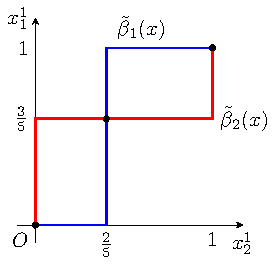
\includegraphics[clip, width=7cm]{./fig/nash_2_1.pdf}
  \caption{最適反応の組}
  \label{fig:nash2}
\end{figure}

\subsection{ナッシュ均衡の存在性}
ナッシュ均衡の存在性を最初に証明したのはNashである.まず,角谷の不動点定理を以下に示す.
\begin{screen}
  \begin{theo}[角谷の不動点定理]
    コンパクトで凸な集合$D \subseteq \mathbb{R}^r$に対し,対応$g:D \to 2^D$が以下の条件を満たすならば,$\exists x^{*} \in g(x^{*})$である.
    \begin{enumerate}
      \item 任意の$x \in D$に対し,$g(x)$が非空で凸.
      \item $g$が上半連続:
      \begin{equation}
        \forall x \in D, \forall 開集合 V \supseteq g(x), \exists 開集合 U, \forall x^{\prime} \in U, g(x^{\prime}) \subseteq V \nonumber
      \end{equation}
    \end{enumerate}
  \end{theo}
\end{screen}

角谷の不動点定理を用いると,ナッシュ均衡の存在性を証明できる.
\begin{screen}
  \begin{theo}
    任意の有限ゲームにおいて,$\exists x^{*} \in \tilde{\beta}(x^{*})$
  \end{theo}
\end{screen}

\begin{proof}
  $X_i$がコンパクトで凸より,$X$もコンパクトで凸.$\forall x \in X$に対して,$\tilde{\beta}_i(x)$は非空で凸より,$\tilde{\beta}(x)$も非空で凸.また,$u_i$の連続性より,$\tilde{\beta}(x)$は上半連続.よって,角谷の不動点定理より,$\exists x \in \tilde{\beta}(x^{*})$.
\end{proof}

ナッシュ均衡の集合$X^{NE}$は,以下の不等式を満たす混合戦略プロファイルとして表現できる.
\begin{equation}
  X^{NE} = \{x \in X \, | \, u_i(x) - u_i(e_i^h, x_{-i}) \geq 0 \; \; \forall i \in \mathcal{N}, \, h \in \mathcal{A}_i\} \label{eq:nash_set}
\end{equation}
\eqref{eq:nash_set}式の右辺の集合は,各多項式が非負になるようなベクトル変数$x$の集合の有限個の共通集合である.代数幾何学の古典的結果から,このような集合は有限個の互いに素な,閉で連結な集合からなるということが導かれる.
これらの集合は,ゲームのナッシュ均衡の成分と呼ばれる.

\begin{theo}
  集合$X^{NE}$は互いに素な,閉で連結な集合の有限和である.
\end{theo}

\subsection{ナッシュ均衡の集合の不変性}
ナッシュ均衡の集合$X^{NE}$は,利得の変化に関して,ある種の不変な性質を持っている.
\begin{screen}
  \begin{theo}
    ナッシュ均衡は,以下の操作に関して不変:
    \begin{enumerate}
      \item 利得関数への正のアフィン変換.
      \item 利得関数の局所シフト.
    \end{enumerate}
  \end{theo}
\end{screen}


定数$\mu_i \in \mathbb{R}$と正の定数$\lambda_i \in \mathbb{R}_{++}$に対して,
\begin{itemize}
  \item 利得関数への正のアフィン変換
  \begin{equation}
    \forall x \in X \; \; \tilde{u}_i(x) = \lambda_i u_i(x) + \mu_i \nonumber
  \end{equation}
  \item 利得の局所シフト
  \begin{equation}
    \forall x \in X \; \; \tilde{u}_i(x) = \begin{cases}
      u_i(x) & \mbox{if} \; \; x_{-i} \neq \bar{x}_{-i} \\
      u_i(x) + \mu_i & \mbox{if} \; \; x_{-i} = \bar{x}_i
  \end{cases}\nonumber
  \end{equation}
\end{itemize}
いずれの場合も
\begin{equation}
  \tilde{u}_i(x_i^{*}, x_{-i}) \geq \tilde{u}_i(x_i, x_{-i}) \Leftrightarrow u_i(x_i^{*}, x_{-i}) \geq u_i(x_i, x_{-i}) \nonumber
\end{equation}
である.

この不変な性質により計算が著しく容易になる場合もある.また,外見上異なるゲームも同じ最適反応対応を持つ.

\subsection{戦略の支配関係}
\begin{screen}
  \begin{defi}
    \begin{itemize}
      \item $x_i^{*} \in X_i$が$x_i \in X_i$を強支配するとは,
      \begin{equation}
        \forall z_{-i} \; \; u_i(x_i^{*}, z_{-i}) > u_i(x_i, z_{-i}) \nonumber
      \end{equation}
      が成り立つときをいう.
      \item $x_i^{*} \in X_i$が$x_i \in X_i$を弱支配するとは,
      \begin{equation}
        \forall z_{-i} \; \; u_i(x_i^{*}, z_{-i}) \geq u_i(x_i, z_{-i}) \; かつ \; \exists z_{-i} \; \; u_i(x_i^{*}, z_{-i}) > u_i(x_i, z_{-i}) \nonumber
      \end{equation}
      が成り立つときをいう.
    \end{itemize}
  \end{defi}
\end{screen}

この定義から,以下のことが分かる.
\begin{itemize}
  \item 強支配される戦略は,いついかなるときも最適にはならない.
  \begin{itemize}
    \item 合理性: 強支配される戦略は使われない.強支配される純粋戦略の消去.
  \end{itemize}
  \item 弱支配される戦略は,最適になることもある.
  \begin{itemize}
    \item いかなる戦略に対しても唯一の最適反応とはならない.
    \item 合理性: 弱支配される戦略の使用は必ずしも否定されない.
  \end{itemize}
\end{itemize}

弱支配されている戦略の組がナッシュ均衡になる例を示す.
\begin{table}[H]
\centering
  \begin{tabular}{c|c|c}
        & L & R  \\ \hline
    T & $1, 1$ & $2, 0$ \\ \hline
    B & $0, 2$ & $2, 2$ \\
  \end{tabular}
\end{table}
上の表について.支配関係を考える.
\begin{itemize}
  \item BはTに弱支配され,RはLに弱支配されている.
  \item 弱支配されている戦略の組,(B, R)もナッシュ均衡である.
\end{itemize}
最適反応は,
\begin{itemize}
  \item Lに対してT,Rに対してTとB.
  \item Tに対してL,Bに対してLとR.
\end{itemize}
である.よって,ナッシュ均衡$x^{*}$は,
\begin{equation}
  x^{*} \in \{(e_2^1, e_2^1), (e_2^2, e_2^2)\} \nonumber
\end{equation}
である.

戦略の反復消去について述べる.

エージェントが合理的に振る舞うということは,各エージェントは自身の利得が最大になるような戦略を取ろうとするということである.ここで,エージェントの共有知識として,以下のようなものを考える.
\begin{enumerate}
  \item 他のエージェントも合理的だと知っている.\label{enu:gr}
  \item 他のエージェントの戦略や利得関数を知っている.\label{enu:gr2}
  \item 他のエージェントが\ref{enu:gr}と\ref{enu:gr2}を知っている.\label{enu:gr3}
  \item 他のエージェントが\ref{enu:gr3}を知っている.
  \item etc...
\end{enumerate}

これを利用して,強支配される戦略の反復消去を行う.
\begin{enumerate}
  \item 自身の強支配される戦略を消去.\label{enu:strong1}
  \item \ref{enu:strong1}後のゲームで,他のエージェントの強支配される戦略を消去.\label{enu:strong2}
  \item \ref{enu:strong2}後のゲームで,自身の強支配される戦略を消去.\label{enu:strong3}
  \item \ref{enu:strong3}後のゲームで,他のエージェントの強支配される戦略を消去.
  \item etc...
\end{enumerate}

これについても具体例で説明する.以下の利得行列を持つ2人ゲームを考える.
\begin{equation}
  A = \left(
  \begin{array}{ccc}
    3 & 1 & 6 \\
    0 & 0 & 4 \\
    1 & 2 & 5
  \end{array}
  \right), \; B = \left(
  \begin{array}{ccc}
    3 & 0 & 1 \\
    1 & 0 & 2 \\
    6 & 4 & 5
  \end{array}
  \right) \nonumber
\end{equation}
\begin{itemize}
  \item エージェント1の戦略1が戦略2を強支配しているので,戦略2を消去.
  \begin{equation}
    A = \left(
    \begin{array}{ccc}
      3 & 1 & 6 \\
      1 & 2 & 5
    \end{array}
    \right), \; B = \left(
    \begin{array}{ccc}
      3 & 0 & 1 \\
      6 & 4 & 5
    \end{array}
    \right) \nonumber
  \end{equation}
  \item エージェント2の戦略1が戦略2と戦略3を強支配しているので,戦略2と戦略3を消去.
  \begin{equation}
    A = \left(
    \begin{array}{c}
      3 \\
      1
    \end{array}
    \right), \; \;
    B = \left(
    \begin{array}{c}
      3 \\
      6
    \end{array}
    \right) \nonumber
  \end{equation}
  \item エージェント1の戦略1が戦略3を強支配しているので,戦略3を消去.
  \begin{equation}
    A = \left(
    \begin{array}{c}
      3
    \end{array}
    \right), \; \;
    B = \left(
    \begin{array}{c}
      3
    \end{array}
    \right)\nonumber
  \end{equation}
\end{itemize}

反復消去により,戦略プロファイルが1つだけ残る.このプロファイルは強ナッシュ均衡である\footnote{反復支配戦略均衡と呼ばれることもある.}.

\begin{screen}
  \begin{defi}
    \begin{itemize}
      \item $x_i^{*}$が全ての$x_i \in X_i$を弱支配するとき,$x_i^{*}$を支配戦略という.
      \item 全ての$i \in \mathcal{N}$に対し,$x_i^{*} \in X_i$が支配戦略ならば,$x^{*} = (x_1^{*}, \ldots, x_m^{*}) \in X$を支配戦略均衡とう.
    \end{itemize}
  \end{defi}
\end{screen}

支配戦略は,他のエージェントの戦略に関わらず合理的である.ただし,存在するとは限らない.支配戦略均衡は,各エージェントが自身の情報のみで到達できるが,存在するとは限らない.支配戦略均衡は明らかにナッシュ均衡の条件を満たす.

\subsection{ナッシュ均衡の特徴}
ナッシュ均衡の長所と短所は以下に挙げられる.
\begin{itemize}
  \item 長所
  \begin{itemize}
    \item エージェントの合理性を元にした自然な解である.
    \item 一旦実現されると,戦略を変更するメリットがない.
    \item 必ず存在する.
  \end{itemize}
  \item 短所
  \begin{itemize}
    \item どのようにナッシュ均衡にたどり着くか考えない.
    \item 複数(時には多数)存在する場合がある.
  \end{itemize}
\end{itemize}
このように考えると,エージェントが選びやすそうなナッシュ均衡であったり,摂動や外乱に対して頑健なナッシュ均衡であるのが好ましい.\ref{sec:refine}節ではナッシュ均衡の精緻化について述べる.

\section{ナッシュ均衡の精緻化}\label{sec:refine}
精緻化とは,特定の信憑性のないナッシュ均衡や壊れやすいナッシュ均衡を排除することを動機としている.以下で,いくつかの標準形精緻化を定義する.

\subsection{完全性}
最もよく知られた非協力精緻化は,「震える手」の完全性という精緻化である.この精緻化は,エージェントの戦略の摂動に対し,頑健でないナッシュ均衡を排除するものである.

ゲームを$G = (\mathcal{N}, X, u)$とし,$\mu$を誤差ベクトルとする.
この誤差ベクトルは,各エージェント$i$と純粋戦略$j \in \mathcal{A}_i$に対して1つの数$\mu_i^j \in (0, 1)$を割り当てる.この数は戦略が「誤って」プレーされる確率であり,$\sum_{j \in \mathcal{A}_i} \mu_i^j < 1$である.
この誤差ベクトル$\mu$に対し,戦略空間の部分空間$X(\mu) = \{x \in X \, | \, \forall i \in \mathcal{N} \; \forall j \in \mathcal{A}_i \; x_i^j \geq \mu_i^j\} \subseteq \mbox{int}(X)$が定義できる.
混合戦略を$X(\mu)$に制限したゲーム$G(\mu) = (\mathcal{N}, X(\mu), u)$を$G$の摂動ゲームと呼ぶ.以下に定義として再掲する.

\begin{screen}
  \begin{defi}
    ある誤差ベクトル$\mu \in \{\mu \in \mathbb{R}_{++}^m \, | \, \forall i \in \mathcal{N} \; \sum_{j \in \mathcal{A}_i} \mu_i^j < 1\}$
    に対し,$X$の部分空間
    \begin{equation}
      X(\mu) = \{x \in X \, | \, \forall i \in \mathcal{N} \; \forall j \in \mathcal{A}_i \; x_i^j \geq \mu_i^j\} \nonumber
    \end{equation}
    を定義する.混合戦略を$X(\mu)$に制限したゲーム
    $G(\mu) = (\mathcal{N}, X(\mu), u)$
    を$G$の摂動ゲームと呼ぶ.ただし,$m = \sum_{i \in \mathcal{N}} m_i$ (すべてのエージェントの戦略の総数) である.
  \end{defi}
\end{screen}

任意の摂動ゲーム$G(\mu)$は非空のナッシュ均衡の集合$X^{NE}(\mu)$を持つ.全ての誤差確率が小さければ小さいほど$X(\mu)$は大きくなり,また,誤差確率がゼロに近づけば対応する摂動ゲームはもとのゲームに近づく.以下で「震える手」の完全性について定義する.

\begin{screen}
  \begin{defi}[完全性]
    ナッシュ均衡$x^{*} \in X^{NE}$が完全であるとは,以下の条件を満たす摂動ゲームの列
    $\{G(\mu^t)\}_{\mu^t \to 0}$が存在することをいう.
    \begin{enumerate}
      \item $x^{t}$が$G(\mu^t)$のナッシュ均衡.
      \item $x^t \to x^{*}$.
    \end{enumerate}
  \end{defi}
\end{screen}

この定義は,エージェントがある微小な確率で誤った戦略を選択しても,元のゲームのナッシュ均衡に近い結果が実現されることを主張している.特に,任意の内部ナッシュ均衡は完全である.$x \in \mbox{int}(X)$に対し,$x \in X(\mu)$を満たす$\mu$が存在する.

考察しているナッシュ均衡が完全であるためには,それがある低い確率の摂動に関して頑健であれば十分であるから,内部ナッシュ均衡が存在しない場合でも,完全ナッシュ均衡は存在する.
完全ナッシュ均衡の集合を$X^{PE}$と書くと,以下の定理が成り立つ.

\begin{screen}
  \begin{theo}
    任意の有限ゲームに対し,$X^{PE} \neq \emptyset$ (完全ナッシュ均衡は存在する).
  \end{theo}
\end{screen}
\begin{proof}
  任意の列$\{G(\mu^t)\}_{\mu^t \to 0}$に対し,各$t$について$x^t \in X^{NE}(\mu^t)$とする.
  $\{x^t\}_{t = 1}^{\infty}$はコンパクト集合$X$の列なので収束する部分列$\{y^s\}_{s = 1}^{\infty}$をもち,その極限$x^{*}$は$x^{*} \in X$を満たす.
  各$s$に対し,$G(\mu^s)$は対応する摂動ゲームである.連続性より,$x^{*} \in X^{NE}$である.
  さらに,$y^s \to x^{*}$かつ,すべての$s$に対して$y^s \in X^{NE}(\mu^s)$であるので,$x^{*}$は完全である.
\end{proof}

ナッシュ均衡が完全であるための必要十分条件がSeltenにより示されている.それは,$x$のあらゆる均衡について,そのなかに$x$がそれに対する最適反応となる,ある内部戦略プロファイル$y$が存在することである.
言い換えると,エージェントは,互いに他のエージェントの戦略について,いくぶん確信が持てない状況でも,そして,そのために小さな正の確率をそのゲームの全ての純粋戦略に割り当てるとしても,きっと彼らはその均衡戦略$x_i$を進んで取ることはしないだろうということである.
さらに,完全ナッシュ均衡が支配されることは決してなく,もしそのゲームにエージェントが2人しかいなければ,その逆も成り立つ.

これを命題として書くと,以下のようになる.
\begin{screen}
  \begin{prop}
    任意の完全ナッシュ均衡$x^{*} \in X^{PE}$は(弱)支配されない.特に2人ゲームでは逆も成り立つ.つまり,2人ゲームの場合は,$x^{*} \in X^{NE}$が支配されないならば,$x^{*} \in X^{PE}$.
  \end{prop}
\end{screen}

\subsection{プロパー性}
完全性の基準は,ある摂動に関してのみ頑健性を要求するが,この摂動が何らかの意味で合理的なものであるという条件は課していない.
これに対し,ある意味で合理的な誤り方の基準を定義する.
\begin{screen}
  \begin{defi}[$\varepsilon$-プロパー性]
    $x^{*} \in X$が$\varepsilon$-プロパーであるとは,
    \begin{equation}
      \forall i \in \mathcal{N}, \; \forall j, \forall k \in \mathcal{A}_i \; \; u_i(e_i^j, x_{-i}^{*}) < u_i(e_i^k, x_{-i}^{*}) \Rightarrow {x_i^{j}}^{*} \leq \varepsilon {x_i^k}^{*} \nonumber
    \end{equation}
    が成り立つことをいう.
  \end{defi}
\end{screen}

この定義は,コストのかからない誤りほど起こりやすいことを表している.
これはエージェントがより損害の大きな誤りを警戒するように振る舞う,合理的な誤り方である.
任意の内部ナッシュ均衡は,任意の$\varepsilon > 0$に対して$\varepsilon$-プロパーである.


\end{document}
